\documentclass[12pt,a4paper,titlepage,onecolumn]{article}
\usepackage[latin1]{inputenc}
\usepackage{amsmath}
\usepackage{amsfonts}
\usepackage{amssymb}
\usepackage{graphicx}
\usepackage{titlesec}
\newcommand{\sectionbreak}{\clearpage}
\author{mkem114 - 6273632}
\title{VOXSpell User Manual}

\begin{document}
	\maketitle
	\tableofcontents
	\listoffigures
	
	\section{Getting Started}
	You might need an adult to help you get started the first time. You need open a terminal; change to the game folder(if not already there), type in "chmod 777 RUN.sh" (without the quote marks), press enter, type in "./RUN.sh" and press enter. Please see Figure ~\ref{fig:TerminalandFolder} for a general look, the green and blue writing is normally different for you as well as the icons and theme.
	\begin{figure}[h]
	\centering
	\includegraphics[width=1\linewidth]{"Figures/Getting Started/TerminalandFolder"}
	\caption[Terminal commands]{General overview of terminal, commands and folder with VOXSpell}
	\label{fig:TerminalandFolder}
	\end{figure}\\
	Please read the "README.txt" as and if there's any problems it may help.
	
	\section{Introduction}
	Welcome to VOXSpell! The best spelling quiz game for New Zealand kids! If you haven't already read the README.txt file please do because it's important.\\
		\subsection{Quitting/Exiting}
		If your parents, teacher or caregiver catch you playing when you're not meant to be or if you're done playing exit the game at any time by pressing the little "X" button normally in the top-right or top-left corners of VOXSpell like in Figure ~\ref{fig:Exit}.
		\begin{figure}[h]
		\centering
		
\includegraphics[width=0.1\linewidth]{Figures/Introduction/Exit}
		\caption[Quit/Exit]{VOXSpell quit/exit button}
		\label{fig:Exit}
		\end{figure}
		\subsection{To Main Menu}
		Most of the time a button called "Menu" will be in the bottom-right corner of VOXSpell that will take you to the main menu if you click on it (see Section ~\ref{mainmenu}).
		\begin{figure}[h]
		\centering
		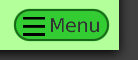
\includegraphics[width=0.2\linewidth]{Figures/Introduction/Menu}
		\caption[Menu Button]{Menu button always goes to the main menu}
		\label{fig:Menu}
		\end{figure}


	
	\section{Picking a Level}\label{picklevel}
	\begin{figure}[h]
	\centering
	\includegraphics[width=1\linewidth]{"Figures/Picking a Level/PickLevelGeneral"}
	\caption[PickLevel]{First run (and reset) screen to pick starting level}
	\label{fig:PickLevelGeneral}
	\end{figure}

	When you run VOXSpell for the first time you will see something like Figure ~\ref{fig:PickLevelGeneral}. This is because you need a level to start from, you should pick a level that isn't too hard and not too easy for you. \\
	You can pick a level by clicking where it says "1" in Figure ~\ref{fig:PickLevelGeneral} and then clicking on the name of the level that you would like to pick. If you would like to hear a word in the level to find out how hard it is then click on the "Preview" button as in Figure ~\ref{fig:PickLevelGeneral}.\\
	Once you picked the level you want to start on click on the "Play" button which will take you to the main menu (see Section \ref{mainmenu}).
	
	\section{Main Menu}\label{mainmenu}
	\begin{figure}[h]
	\centering
	\includegraphics[width=1\linewidth]{"Figures/Main Menu/MainMenuGeneral"}
	\caption[Main Menu]{The main menu}
	\label{fig:MainMenuGeneral}
	\end{figure}
	After a level has been picked or if the game is run again (not for the first time) then this screen like in Figure ~\ref{fig:MainMenuGeneral} will appear; this is the main menu. To play a new quiz click on the "Play" button. To play any level or add your own levels or your own words click on the "Custom" button. To see your game scores click on "Statistics". To change the voice or reset the game click on the "Options" button. 
	\subsection{Background Music}
	To pause the background music that plays everytime you go to the main menu click on the "Music" button and to start it playing it again click on "Music" again. When you leave the main menu the music stops playing so you can hear the speaker. To change the music look in the README.txt
	
	\section{Playing a Quiz}\label{quiz}
	This mode starts you on your picked starting level. All levels with names that are numbers(integers) can be played and when you finish a level you move on to the next one. You can add more levels or add more words to play in Section ~\ref{addlist}. When you first click on "Play" in the main menu you will see Figure ~\ref{fig:NewQuizStart}
	\begin{figure}[h]
	\centering
	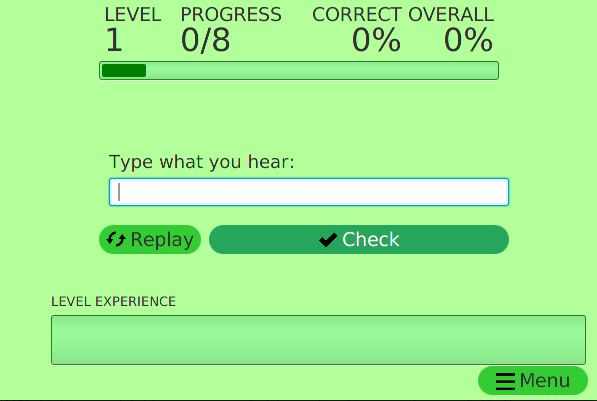
\includegraphics[width=1\linewidth]{Figures/NewQuiz/NewQuizStart}
	\caption[Quiz Start]{Start of a new quiz and level}
	\label{fig:NewQuizStart}
	\end{figure}
		\subsection{Statistics}
		"LEVEL" is the level you are playing. "PROGRESS" is how many words you have played this quiz and how many are in the quiz. "CORRECT" is how many words you have gotten right first go this quiz out of all the words you have played this quiz as a percentage. "OVERALL" is how many first goes were right out of all first goes you've played on this level as a percentage. The green bar below all of these is how far through the quiz you are. Figure ~\ref{fig:NewQuizFirstWordRight} is different to Figure ~\ref{fig:NewQuizStart} because the player answered the first word right on the first go.
		\begin{figure}[h]
		\centering
		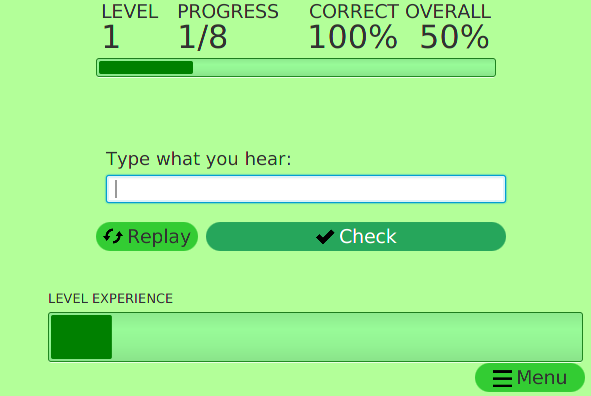
\includegraphics[width=1\linewidth]{Figures/NewQuiz/NewQuizFirstWordRight}
		\caption[Right First Word]{The first word was answered right on the first go}
		\label{fig:NewQuizFirstWordRight}
		\end{figure}
		\subsection{Playing}
		The game randomly picks words from the level you're on and is more likely to pick words which you need to work on or have played less.\\
		For every word in the quiz the game will say the word through the speaker to you, you type where it says "Type what you hear..." and click the "Check" button when you're done. If you spelt the word correctly you will have mastered the word (then go to the next word), if you spell it wrong then the game will tell you and you'll get another chance to spell the word. If you spell it right then you faulted the word and if it is wrong again you have failed the word. If you failed the word then game will tell you the right spelling for the word and you must press the "OK" button to go to the next word (see Figure ~\ref{fig:NewQuizSecondWordWrong}).
		\begin{figure}[h]
		\centering
		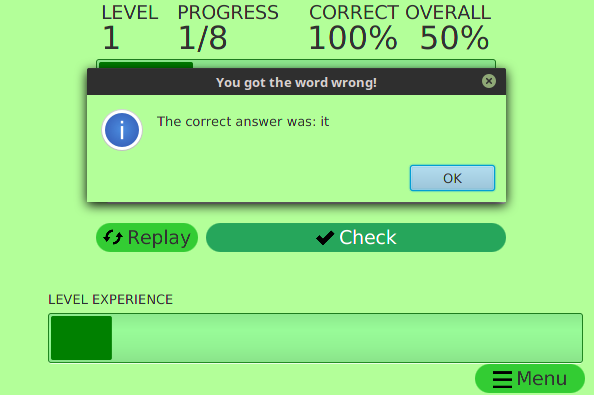
\includegraphics[width=1\linewidth]{Figures/NewQuiz/NewQuizSecondWordWrong}
		\caption[Failed Word]{The player spelt the word wrong twice}
		\label{fig:NewQuizSecondWordWrong}
		\end{figure}\\
		If you didn't hear the word you can press the "Replay" button and the game will say the word to you again.
		\subsection{Experience}
		To move on to the next level you need to have mastered all the words in the level at least once and you might need to do more than one quiz to do it. The big green bar at the bottom of the screen will grow the closer you get to the next level (see the difference in the bottom bar when the player mastered a word in Figure ~\ref{fig:NewQuizFirstWordRight} versus Figure ~\ref{fig:NewQuizStart}).
		\subsection{End of Quiz}
		Once you have answered all the words in the quiz you will come to the end of the quiz which looks like Figure ~\ref{fig:NewQuizEndNoReward} unless you unlocked the video reward like in Figure ~\ref{fig:NewQuizEndReward}. The "Score" is how many words in the quiz you mastered out of how many words were in the quiz and the "All-time" is all the mastereds you got in the level out of all goes at words in the level as a percentage. If you got 90\% or more words mastered in the quiz you get the "Video Reward" button which if clicked on takes you to the video reward.\\ If you got your experience bar to the end then the "Continue" button takes you to a new quiz on the next level otherwise it takes you to a new quiz on the same level.
		\begin{figure}[h]
		\centering
		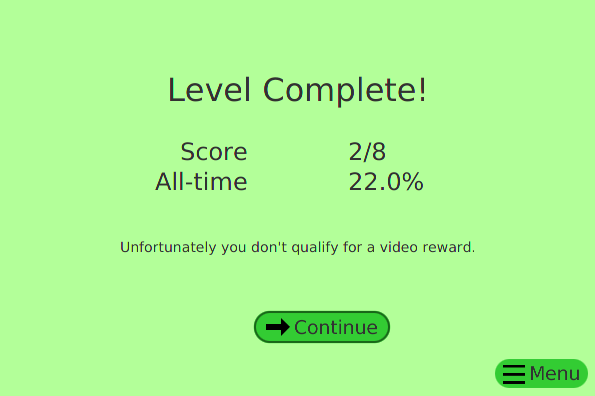
\includegraphics[width=1\linewidth]{Figures/NewQuiz/NewQuizEndNoReward}
		\caption[Quiz End without Reward]{The player finished the quiz and didn't get the video reward}
		\label{fig:NewQuizEndNoReward}
		\end{figure}
		\begin{figure}[h]
			\centering
			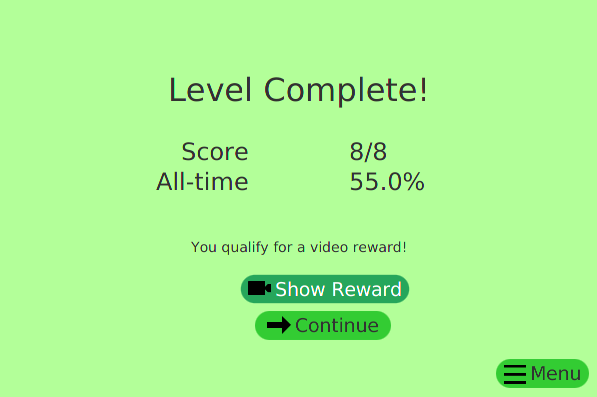
\includegraphics[width=1\linewidth]{Figures/NewQuiz/NewQuizEndReward}
			\caption[Quiz End with Reward]{The player finished the quiz and got the video reward}
			\label{fig:NewQuizEndReward}
		\end{figure}
			\subsubsection{Video Reward}
			\begin{itemize}
				\item The "5s" button on the left will take the video back 5 seconds.
				\item The "Play" button will start the video and become a "Pause" button. When "Paused" is clicked the video pauses like in Figure ~\ref{fig:VideoRewardPaused}.
				\item The "Stop" button will take the vide to the beginning like when the video reward first opened and in Figure ~\ref{fig:VideoRewardStart}.
				\item The "5s" button on the right will take vide forward 5 seconds.
				\item The "Back" button in the bottom-right corner will go back to the end of the quiz like in Figure ~\ref{fig:NewQuizEndReward}.
			\end{itemize}
			\begin{figure}[h]
			\centering
			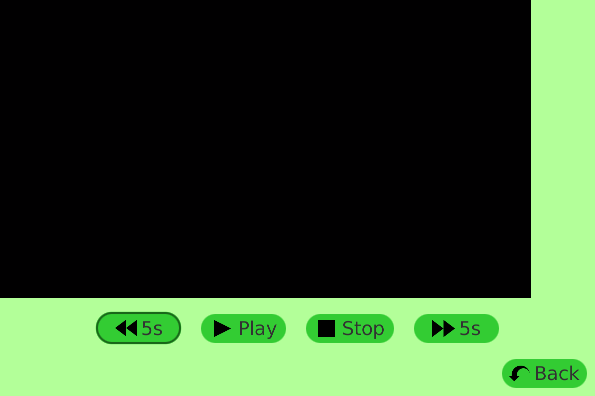
\includegraphics[width=1\linewidth]{Figures/NewQuiz/VideoReward/VideoRewardStart}
			\caption[Video Reward Start]{The player achieved a video reward and opened it}
			\label{fig:VideoRewardStart}
			\end{figure}
			\begin{figure}
			\centering
			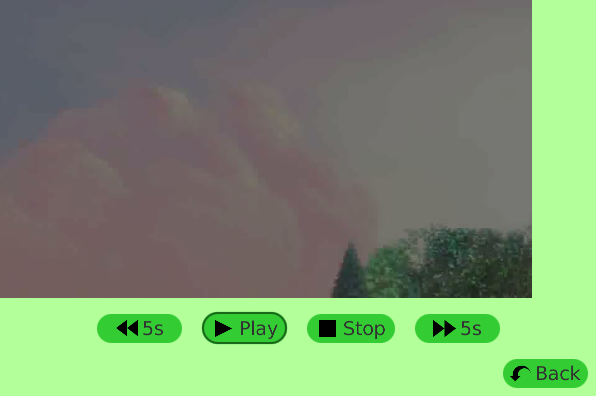
\includegraphics[width=1\linewidth]{Figures/NewQuiz/VideoReward/VideoRewardPaused}
			\caption[Video Reward Paused]{The player achieved a video reward, played it then paused it}
			\label{fig:VideoRewardPaused}
			\end{figure}


	\section{Playing a Custom Quiz}
	Custom quizzes are a lot like non-custom quizzes so please read Section ~\ref{quiz} first. Only what is different will be covered here which is mostly the custom level picker in Section ~\ref{addlist}
		\subsection{Experience}
		There is no experience bar in custom quizzes but times words are mastered, failed and faulted still count like in Figure ~\ref{fig:CustomQuiz}.
		\begin{figure}[h]
		\centering
		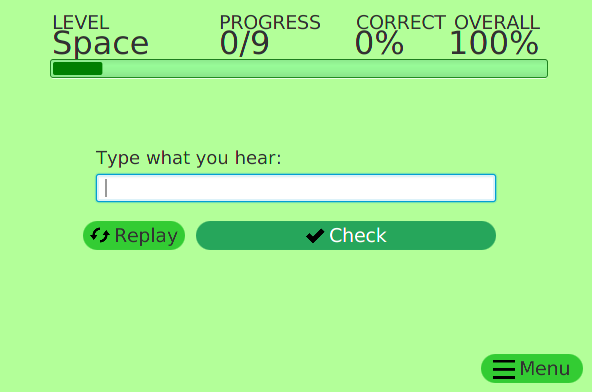
\includegraphics[width=1\linewidth]{Figures/CustomQuiz/CustomQuiz}
		\caption[Custom Quiz]{The user is playing a custom quiz game}
		\label{fig:CustomQuiz}
		\end{figure}
		\subsection{Adding Levels or Words}\label{addlist}
		Because any level can be played in a custom quiz you need to pick one to play.\\ More words or levels can be added the "Open" button in the level picker (Figure ~\ref{fig:CustomLevelPicker}). The text file picked must have the start of a new level being \%Level Name on a new line so that "Name" would be the name of the new level. Any words in the level go on their own new line each below the name of the level. To add more words to a level make the level name the level you want to add words to. Any levels with names that are numbers(integers) will also come up in the non-custom quiz as unlockable and playable levels.
		\begin{itemize}
			\item The picked level name ("Space" in Figure ~\ref{fig:CustomLevelPicker}) when clicked gives you a list of levels to pick from, to see more scroll and then click on the name of the level you want to pick
			\item "Prieview" button randomly picks a word from the level and says it so you can hear how hard the level is.
			\item "Play" button starts a new custom quiz with the picked level.
			\item "Open" button lets you pick a file to add more words or levels.
		\end{itemize}
		\begin{figure}[h]
		\centering
		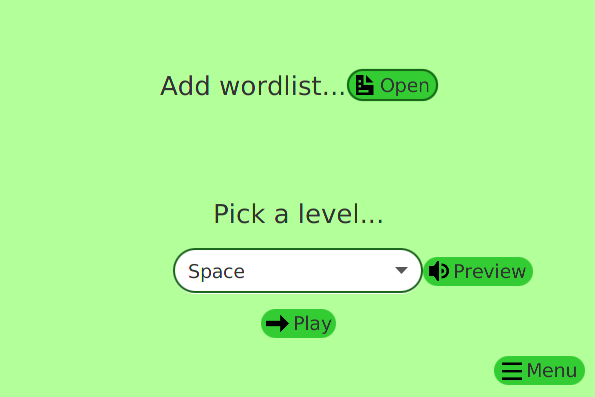
\includegraphics[width=1\linewidth]{Figures/CustomQuiz/CustomLevelPicker}
		\caption[Custom Level Picker]{The player is picking the level to play in their custom quiz}
		\label{fig:CustomLevelPicker}
		\end{figure}
		\subsection{End of Custom Quiz}
		"Continue" button when clicked takes you back to custom level picker (see Section ~\ref{addlist}).
		
	\section{Viewing Statistics}
	\begin{figure}[h]
	\centering
	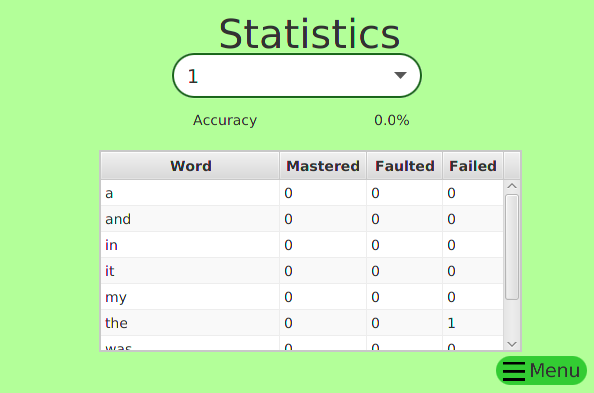
\includegraphics[width=1\linewidth]{Figures/Statistics/StatisticsGeneral}
	\caption[Statistics Menu]{Statistics for each level and each word}
	\label{fig:StatisticsGeneral}
	\end{figure}
	This menu shows you statistics for each level overall and for each word in the level. By default the table of words is sorted alphabetically (like a dictionary).
		\subsection{Levels}
		To pick a level to look at statistics click on the "1" like in Figure ~\ref{fig:StatisticsGeneral} and then click on the level you want to pick; you may need to scroll to see the level you want.\\ The "Accuracy" is the how many words you got right on the first go compared to how many goes you've had as a percentage. \\The table below is all the words in the picked level. "Mastered" is how many times you got the word right on the first go; "Faulted" is how many times you got the word right on the second go and "Failed" is how many times you got the word wrong.
		\subsection{Sorting}
		The table can be sorted or reverse sorted by clicking on "Word", "Mastered", "Faulted" or "Failed" (see Figure ~\ref{fig:StatisticsFailedSorted1}). This will then sort the table of words by what you clicked, if you click again then the way it sorts is reversed (see Figure ~\ref{fig:StatisticsFailedSorted2}).
		\begin{figure}[h]
			\centering
			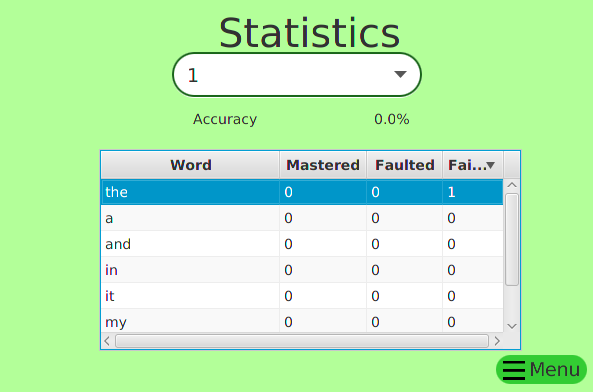
\includegraphics[width=1\linewidth]{Figures/Statistics/StatisticsFailedSorted1}
			\caption[Sorted by Failed]{Statistics word table sorted by number times words were failed}
			\label{fig:StatisticsFailedSorted1}
		\end{figure}
		\begin{figure}[h]
			\centering
			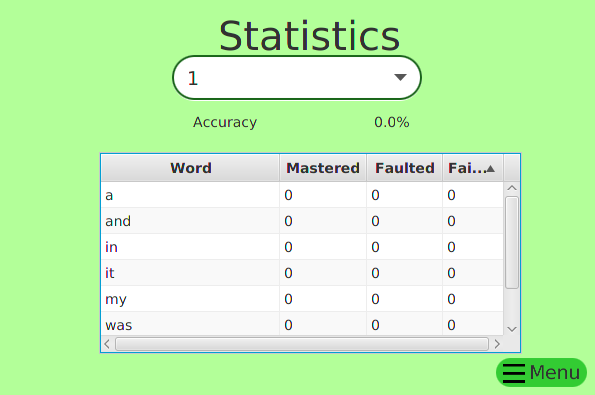
\includegraphics[width=1\linewidth]{Figures/Statistics/StatisticsFailedSorted2}
			\caption[Reverse Sorted by Failed]{Statistics word table reverse sorted by number times words were failed}
			\label{fig:StatisticsFailedSorted2}
		\end{figure}
		
	\section{Changing Options}
		\begin{figure}[h]
		\centering
		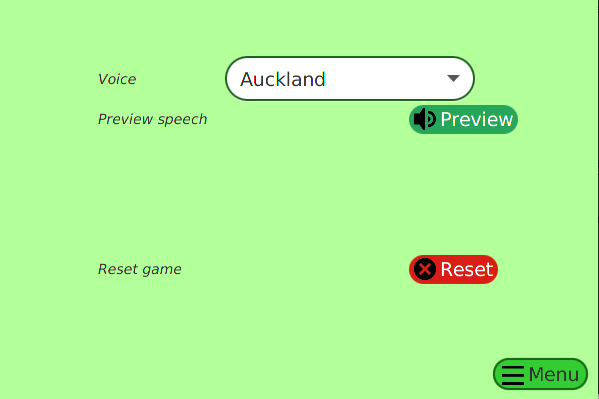
\includegraphics[width=1\linewidth]{Figures/Options/OptionsGeneral}
		\caption[Options Menu]{Options to change voice and reset game}
		\label{fig:OptionsGeneral}
		\end{figure}
		\subsection{Voices}
		To change voices click on the picked voice name ("Auckland" if not changed; see Figure ~\ref{fig:OptionsGeneral}) then click on the voice name you would like to pick ("RAB", "KAL" or "Auckland"). You can hear the voice by clicking the "Preview" button. The "Auckland" voice sometimes won't say a word if it doesn't know how to, try "KAL" or "RAB" if playing hard words.
		\subsection{Reset}
		Clicking the "Reset" button (Figure ~\ref{fig:OptionsGeneral}) will be like starting the game for the first time; you will be taken to pick a starting level (see Section \ref{picklevel}). All scores, any added words and any added levels will be gone. Be very sure before clicking, you might want to ask an adult if this is what you want to do. Sometimes problems with the game go away if the game is reset.
		
\end{document}